\usepackage[utf8]{inputenc}
\usepackage{slovak}
\usepackage{tikz}
\usepackage{fancybox}
\usepackage[english]{babel}
\uselanguage{English}
\languagepath{English}
\usetikzlibrary{arrows,positioning}
\usetheme{Warsaw}
\bibliographystyle{apalike}
\title{Decidability of Termination Problems for Sequential P Systems with Active Membranes}
\author{Michal Kováč}
\institute{FMFI UK, Slovakia}
\date{2.7.2015}
\begin{document}

\begin{frame}[t]
\titlepage
\end{frame}
\note{}

\section*{Outline}
\begin{frame}
\tableofcontents
\end{frame}
\note{}

\section{P systems} % (fold)
\label{sec:p_systems}

  \subsection{Overview} % (fold)
  \label{sub:overview}

    \begin{frame}[t]\frametitle{Membrane structure}
      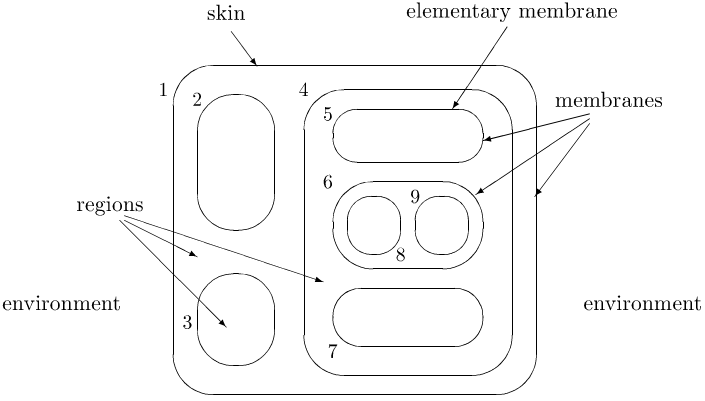
\includegraphics[width=0.7\textwidth]{membrane_structure.png}
      \hfill
      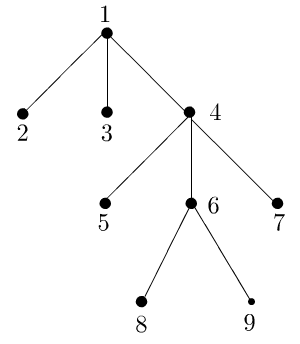
\includegraphics[width=0.3\textwidth]{membrane_tree.png}
      \pause
      \begin{itemize}
        \item Multisets
        \pause
        \item Rewriting rules
        \pause
        \item Passive vs. Active
      \end{itemize}

    \end{frame}
    \note{}

    \begin{frame}[t]\frametitle{P system with active membranes}
    \begin{itemize}
      \item $\Pi = (\Sigma, C_0, R_1, \ldots R_m)$
      \pause
      \item $C = (T, l, c)$
      \begin{itemize}
        \item $l: V(T) \rightarrow \{1, \ldots, m\}$
        \item $c: V(T) \rightarrow \mathbb{N}^\Sigma$
      \end{itemize}
      \pause
      \item Rewriting rules
      \begin{itemize}
        \item $u\rightarrow v$
        \item $u\rightarrow v\delta$
        \item $u\rightarrow [_j v]_j$,

        where $u \in \mathbb{N}^\Sigma, |u|\geq 1$ and $v\in \mathbb{N}^{\Sigma\times\{\cdot, \uparrow, \downarrow_{j}\}}$
      \end{itemize}

    \end{itemize}
    \end{frame}
    \note{}

    \begin{frame}[t]\frametitle{Computation}
      \begin{itemize}
        \item Maximal parallel vs. sequential
        \pause
        \item Language
        \begin{itemize}
          \item generating mode
          \item accepting mode
        \end{itemize}
      \end{itemize}

    \end{frame}
    \note{}

  % subsection overview (end)

  \subsection{Computational power} % (fold)
  \label{sub:computational_power}
    
    \begin{frame}[t]\frametitle{Chomski hierarchy}
      \begin{tikzpicture}
        \node(reg){REG};
        \node[right=2cm of reg](cf){CF};
        \node[right=2cm of cf](cs){CS};
        \node[right=2cm of cs](re){RE};
        \path[-triangle 45] (reg) edge (cf);
        \path[-triangle 45] (cf) edge (cs);
        \path[-triangle 45] (cs) edge (re);
        \pause
        \node[below=1cm of cs](et0l){ET0L};
        \path[-triangle 45] (cf) edge (et0l);
        \path[-triangle 45] (et0l) edge (re);
        \pause
        \node[below=2cm of et0l](petri){Petri nets};
        \path[-triangle 45] (reg) edge (petri);
        \path[-triangle 45] (petri) edge (re);
        \pause
        \node[below=0.3cm of cf](seqncoo){seq, non-coo};
        \node[below=0.3cm of et0l.west](maxparncoo){max-par, non-coo};
        \node[right=0.3cm of re.south](maxparcoo){max-par, coo};
        \pause
        \node[below=0.3cm of petri](seqcoo){seq, coo};
        \pause
        \node[below=0.1cm of maxparcoo](seqactcoo){seq, coo, active};
        \pause
        \node[below=0.1cm of seqactcoo](citeibarra){\cite{Ibarra05Active}};
      \end{tikzpicture}
      
    \end{frame}
    \note{}

    % subsection computational_power (end)

% section p_systems (end)

\section{Termination problems} % (fold)
\label{sec:termination_problems}

  \subsection{Halting problem} % (fold)
  \label{sub:halting_problem}
  
    \begin{frame}[t]\frametitle{Termination problems}
      \begin{itemize}
        \item Halting problem
        \pause
        \item Existence of (in)finite computation
        \pause
        \item Reachability graph
        \pause
        \item Two conditions:
        \begin{itemize}
          \item $C_1 \leq C_2 \Rightarrow$ each transition in $C_1$ can be fired in $C_2$
          \pause
          \item for each infinite computation there is $C_1, C_2$, such that $C_1 \rightarrow^* C_2$ and $C_1 \leq C_2$
        \end{itemize}
        \pause
        \item Dickson's lemma: For every infinite sequence of tuples over $\mathbb{N}$ $\{a_i\}_{i=0}^\infty$ there are $i<j$ such that $a_i\leq a_j$
      \end{itemize}

    \end{frame}
    \note{}


  % subsection halting_problem (end)

  \subsection{Termination problems in active membranes} % (fold)
  \label{sub:termination_problems_in_active_membranes}

    \begin{frame}[t]\frametitle{Termination problems in active membranes}
      \begin{itemize}
        \item How to use Dickson's lemma for active membranes?
        \item Idea: encode configuration to k-tuple maintaining two conditions
      \end{itemize}
      \pause

      \begin{definition}
        $C_1 = (T_1, l_1, c_1) \leq C_2 = (T_2, l_2, c_2) \Leftrightarrow$
      
        $\exists \text{~isomorphism~} f: T_1\rightarrow T_2 \text{~such that~}\forall d\in V(T_1):$
        \begin{itemize}
          \item $l_1(d) = l_2(f(d))$
          \item $c_1(d) \subseteq c_2(f(d))$
        \end{itemize}
      \end{definition}
      \pause
      
      \begin{lemma}
        $C_1 = (T_1, l_1, c_1) \leq C_2 = (T_2, l_2, c_2) \Rightarrow \exists \text{~isomorphism~} f: T_1 \rightarrow T_2$

        such that rule $r$ is applicable in $d\in T_1 \Rightarrow r$ is applicable in $f(d)$.
      \end{lemma}
    \end{frame}

    \begin{frame}[t]\frametitle{Termination problems in active membranes}
      \begin{definition}
        Define $enc(C)$ as k-tuple satisfying $enc(C_1)\leq enc(C_2) \Rightarrow C_1\leq C_2$.
      \end{definition}
      \pause

      \begin{lemma}
        For every infinite computation there is $i<j$ such that $C_i\leq C_j$.
      \end{lemma}
      \pause

      \begin{proof}
        Assume infinite sequence $\{enc(C_i)\}_{i=0}^\infty$. From Dickson's lemma there is $i<j$ such that $enc(C_1)\leq enc(C_2)$. Our property of $enc$ implies $C_i\leq C_j$. 
      \end{proof}
    \end{frame}

    \begin{frame}[t]\frametitle{Termination problems in active membranes}
      \begin{theorem}
        Existence of infinite computation in sequential P systems with active membranes is decidable.
      \end{theorem}
      \pause

      \begin{theorem}
        Existence of finite computation in sequential P systems with active membranes is undecidable.
      \end{theorem}
      \pause

      \begin{proof}
        Reduction to reachability of register machines.
      \end{proof}
    \end{frame}

  % subsection termination_problems_in_active_membranes (end)

% section termination_problems (end)

\begin{frame}[plain]
  \bibliography{cie}
\end{frame}


\begin{frame}[plain]
  \begin{center}
    Thanks for your attention!
  \end{center}
\end{frame}

\end{document}
